%% LaTeX template for BSc Computing for Games final year project dissertations
%% by Edward Powley
%% Games Academy, Falmouth University, UK

%% Based on:
%% bare_jrnl.tex
%% V1.4b
%% 2015/08/26
%% by Michael Shell
%% see http://www.michaelshell.org/
%% for current contact information.
%%
%% This is a skeleton file demonstrating the use of IEEEtran.cls
%% (requires IEEEtran.cls version 1.8b or later) with an IEEE
%% journal paper.
%%
%% Support sites:
%% http://www.michaelshell.org/tex/ieeetran/
%% http://www.ctan.org/pkg/ieeetran
%% and
%% http://www.ieee.org/

%%*************************************************************************
%% Legal Notice:
%% This code is offered as-is without any warranty either expressed or
%% implied; without even the implied warranty of MERCHANTABILITY or
%% FITNESS FOR A PARTICULAR PURPOSE! 
%% User assumes all risk.
%% In no event shall the IEEE or any contributor to this code be liable for
%% any damages or losses, including, but not limited to, incidental,
%% consequential, or any other damages, resulting from the use or misuse
%% of any information contained here.
%%
%% All comments are the opinions of their respective authors and are not
%% necessarily endorsed by the IEEE.
%%
%% This work is distributed under the LaTeX Project Public License (LPPL)
%% ( http://www.latex-project.org/ ) version 1.3, and may be freely used,
%% distributed and modified. A copy of the LPPL, version 1.3, is included
%% in the base LaTeX documentation of all distributions of LaTeX released
%% 2003/12/01 or later.
%% Retain all contribution notices and credits.
%% ** Modified files should be clearly indicated as such, including  **
%% ** renaming them and changing author support contact information. **
%%*************************************************************************


\documentclass[journal]{IEEEtran}

\usepackage{graphicx}
% Insert additional usepackage commands here

\begin{document}
%
% paper title
% Titles are generally capitalized except for words such as a, an, and, as,
% at, but, by, for, in, nor, of, on, or, the, to and up, which are usually
% not capitalized unless they are the first or last word of the title.
% Linebreaks \\ can be used within to get better formatting as desired.
% Do not put math or special symbols in the title.
\title{How Do Differing Input Methods Impact Player's Ability During Competitive Play in Fighting Games?}
%
%
% author name
\author{Jack Maber - JM192929}

% The paper headers -- please do not change these, but uncomment one of them as appropriate
% Uncomment this one for COMP320
\markboth{COMP320: Research Review and Proposal}{COMP320: Research Review and Proposal}
% Uncomment this one for COMP360
% \markboth{COMP360: Dissertation}{COMP360: Dissertation}

% make the title area
\maketitle

% As a general rule, do not put math, special symbols or citations
% in the abstract or keywords.
\begin{abstract}
Needs filling
\end{abstract}

\section{Introduction}
% The very first letter is a 2 line initial drop letter followed
% by the rest of the first word in caps.
% 
% form to use if the first word consists of a single letter:
% \IEEEPARstart{A}{demo} file is ....
% 
% form to use if you need the single drop letter followed by
% normal text (unknown if ever used by the IEEE):
% \IEEEPARstart{A}{}demo file is ....
% 
% Some journals put the first two words in caps:
% \IEEEPARstart{T}{his demo} file is ....
% 
% Here we have the typical use of a "T" for an initial drop letter
% and "HIS" in caps to complete the first word.
\IEEEPARstart{T}{his} project looks at the impact of the use different input devices during competitive play in "arcade style" fighting games. With the arcade stick being heralded as the superior control scheme by the majority of the FGC (Fighting Game Community)\cite{stickvspad}, there is very little scientific evidence and research that has taken place to support the claims being made, as will be discussed in section II. This paper looks at how the ergonomics of the input methods, as well as the players' skill and anthropometrics impact on the usability of said input methods at an individual level. The use of my programming component and other research techniques that I'll be employing during my research will allow me to the keep track of the inputs that the players are making during game play, which will grant me a better understanding of the overall usability of the input methods and allow me to create a much more informed conclusion. The results will be analysed in section ?. As section II shows, there is a lot of research into the overall usability of different controllers, more innately how the differing anthroprometrics of the users can impact on the usabilty of the controllers. However there is little exploring how it impacts on players' ability during gameplay, and what little there is only covers it from a non-competitive standpoint. The potential conclusions from this study could potentially be used in the games industry to better design input methods so that they support better competitive play for the end users. As well as help users in the competitive scene pick an input method which is scientifically proven to be better matched to them personally. 

\section{The Research Question}
I have chosen my particular research question as I feel it is articulates exactly what I want my research to focus on, rather than focus on game specific exploits (SOCD's) that can give player's an edge, as most of these are either outlawed by the use of input scrubbing devices at competitive events anyway \cite{socdinput}, then add to the fact that players need prior knowledge of these exploits to carry them out, measuring their effectiveness during competitive play with players of different skill levels would be pointless. Whereas focusing on the different input methods most commonly used at competitive events (Game Pads and Arcade Sticks), the data retrieved during my research will hopefully be able to actually show the differences that the input methods display during play and how they affect player's standings, along with how players of differing skill levels adapt to them. 

\section{Related Work and Research}
As the main focus of this paper is on input methods, and how different users interact with them, this will be the primary focus of the related work section. The first section will cover the ergonomic qualities of game controllers and how players interact with them. This primarily because this where the bulk of the existing research focuses on. The following section will be looking more at the historical background of the input methods, as this is a point there is brought up a lot by the FGC that arcade sticks are the most prevalent and superior input method as that's what was around in arcades in the 80s and 90s, when fighting games were at there most popular. The last section will be on the skill aspect, players who have more experience with fighting game will obviously be better and produce more consistent results, but as I want to focus more on the input methods, additional information on the subject will be useful to allow me draw more informed conclusions, and better analyse my data. 

\subsection{Ergonomics, usability and their impact on users} \label{A*PF}
The ergonomics of an input method must meld well with the anthroprometrics of the user to ensure that it is usable and accurate while playing games, a controller that is not intuitive, and causes a heightened amount of frustration to use for a user is one that they will not want to use\cite{brown2013evaluating}. However nowadays most controllers are clearly designed with ergonomics in mind, which Bhardwaj\cite{omichands} goes into heavily by looking in great detail at a number of controllers which show the evolution of the inclusion of ergonomic data in controller design, with the first controller studied, the Mega Drive/Genesis controller, which failed on more criterion than more recent controllers such as the PS4 controller and the Xbox 360, it is heralded as one of the greatest controllers of all time\cite{top25} due to the six button layout of the controller that allowed it greater flexibility when it came to playing a wider variety of games. However as mentioned earlier, the Mega Drive controller failed on more criterion than the much more recently designed controllers, this was mainly down to the fact that the Mega Drive was released in a time period where most games were still played from a 2D perspective, so only a few inputs were needed, due to the decreased complexity\cite{6000321,megadrive}, whereas controllers today need to play a wide variety of different genres, from a number of different perspectives so they must "well suited to play a wide variety of different game styles"\cite{brown2013evaluating}, which can be seen in(fig. \ref{fig:timeline}).

\begin{figure}
    \centering
    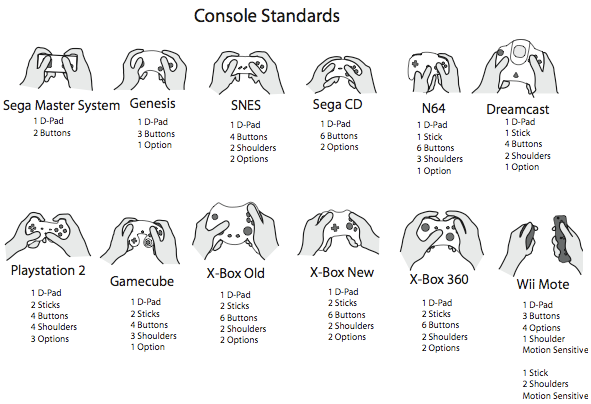
\includegraphics[width=1.0\linewidth]{evolution_of_gamecontroller.png}
    \caption{Controller Evolution Timeline sourced from https://www.back2.co.uk/blog/ergonomics-a-brief-history/}
    \label{fig:timeline}
\end{figure}

Which is a good point to link into what Gerling et al\cite{Gerling:2011:MIG:2181037.2181052} states in saying that the user experience is linked to relevant the controller is they are using, to the game that they are playing. So, it would make sense that controllers for more recent consoles would be heavily influenced by set ergonomic standards such as those proposed by Tilley\cite{tilley}, which is the exact standard that Bhardwaj\cite{omichands} used when studying his selection of input devices, as these best showed the evolution of ergonomic design choices over time when it came to game controllers, and the standards set by Tilley also outline the optimum dimensions and actuation force for things such as buttons and triggers, so it makes perfect sense to use these figures as a benchmark, as they represent the "50th" percentile\cite{omichands} with this group of people represent the group with the most average anthroprometrics, while the 5th and 9th percentile have metrics that either too small or too large to fit into the average. Therefore it is important for designers to create parts for a controller to cover the widest possible set of metrics\cite{heatherly2014video}, however this can be quite difficult when metrics such as hand size can vary from 13 - 19 cm as Brown et al found\cite{brown2013evaluating}. As the anthroprometrics of users can vary so wildly, and hand size is seemingly the most important metric to take into account when designing a controller, it is important that controllers are small enough so that players in the 5th percentile can reach all of the buttons (Which was the main problem with the original Xbox controller, better known as the "Duke" because of it's size\cite{omichands}), while users in the 95th percentile can still activate all the inputs easily, without additional accidental input. To further cement the fact that the controllers that clearly designed with ergonomics in mind should in theory allow users to perform better due to increased comfort and usability\cite{brown2013evaluating}, this relation has also been found in other fields such as medical equipment, where Berguer et al\cite{berguer2004relationship} found that medical professionals using surgical instruments also had significant trouble using the instrumentation when they had hands smaller than a size six and half glove, which equates to roughly 36 percent of surgeons at the time of the research. More interesting than that though is that of the 36 percent, 87 percent of the surgeons that had significant were women, this claim is definitely valid as Tilley et al found that on average woman's hands were 13cm less across than men's\cite{tilley}.


This is a very interesting statistic on many fronts when drawing a parallel over to talking about both video games and usability, as there are is plenty of evidence to suggest that the number of women playing video games has been on a relatively steady increase since 2006\cite{genderdistribution2006}, however the increase was mostly prevalent within the mobile gaming sector\cite{gameanalyticswomen}, with Google finding that over 64 percent of women preferred mobile gaming over other gaming platforms\cite{womenmobilegaming}, this increase may be caused by the sharp uptake of mobile devices in general, however the relationship between more women taking up playing games and the rise in popularity is extremely clear(fig. \ref{fig:smartphone}). As games on mobile are normally much simpler due to the fact the hardware is a lot less powerful than regular home consoles, they normally fall more into the "casual" genre, which gives them the ability to be picked up and played in short sessions, and due to the fact that the only form of input on a mobile device is through the touch screen, this limits the ceiling of complexity that a game can have, compared to that of a console game. So they must be both intuitive and easy to control. And as Google found\cite{womenmobilegaming}, women mostly play to relieve stress or fill an empty moment, which is pretty telling that they prefer to use games as more of a time killing tool, rather than playing it for reasons such as the story or a competitive aspect, which is why, as stated before, mobile games are normally fit more into the "casual" part of the market.

\begin{figure}
    \centering
    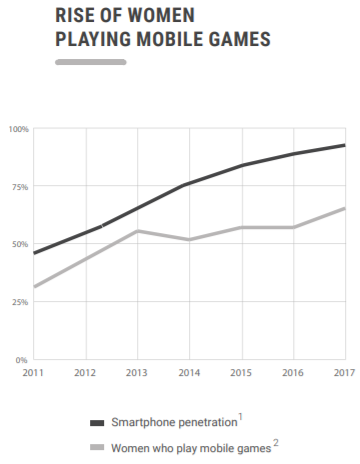
\includegraphics[width=0.5\linewidth]{smartphone.PNG}
    \caption{Graph showing the rise in popularity of smart devices and women who play mobile games \cite{womenmobilegaming}}
    \label{fig:smartphone}
\end{figure}

So as such, even though there has been an increase in women playing video games, they are still very much under represented in more competitive games, especially in fighting games, which is extremely evident when looking at articles from within the FGC, all of the articles about the few female players who have been interviewed note that they play in a very much male dominated community\cite{sooa}, with many facing "getting harassed, made fun of, objectified"\cite{comboqueens} which would definitely prevent women from becoming more involved in the community. However I also feel that this will affect how future input devices will be created for fighting games such as the arcade stick will be designed, as other popular games that are heavily grounded in E-sports such as League Of Legends have had all female pro teams at points\cite{femalelol}, are all based on PC, and thus the peripheral market has expanded to include input methods that cater to users with smaller hands, such as those possessed by women, mouse manufacturers such as Zowie produce some of their popular E-sports mice in 3 different sizes\cite{zowiemouse} to cater to a wider audience of users. However the input devices that the main input device that this study will be focusing on, the arcade stick, although the sizes of the actual devices outside dimensions can vary wildly, the button layout is normally, at least for professional Street Fighter, a set layout most commonly the same as visible in(fig. \ref{fig:buttonlayout}). Having a set panel layout, although making the device easy to remember once learnt and easy to produce, it's usability can depend on the size of the users hands, and how comfortable they find the orientation of the buttons, along with how familiar they are with the controller, and although these factors also transfer to the other input methods that this paper will be studying, due to the relative obscurity of the arcade stick, I feel that it will be the least user friendly compared to the other devices as participants who don't have much experience with video games will have mostly likely used one of the more conventional input devices in the past. Due to the amount of impact that the ergonomics of the input methods can have, and the vast differences in the anthroprometrics of users that I found in this section, I'll be taking a closer look at the input methods this paper will be covering in the next section to gain a better idea of their history and most common usages.   

\subsection{The researched input methods, and their place in the community} \label{A*PF}
There are two prevalent input methods that are used in the fighting game community, the arcade stick and the "pad". The arcade stick is held in very high regard in the FGC, and is considered almost the "default" controller for nearly all fighting games\cite{Su:2010:SFI:1718918.1718981} except for 3D fighters such as Tekken and Soul Calibur as their predominant controller is a Playstation pad due to the design of the D-pad\cite{controllerchoice} as the reduced range of motion compared to an arcade stick makes changing direction quicker, as this is much more important in 3D fighter due to the added dimension of movement. The GameCube controller is used almost primarily in the Smash Brothers community, especially for Melee, which was the first game in the series to be launched on the GameCube and the first to gather a competitive community, even though there is a lot of disagreement within the wider FGC that if Smash should even be classed as a fighting game due to the sheer amount of restrictions that are enforced on the game to enable it to function as a competitive game, due to mostly the fact that features such as the items that appear during gameplay, and the stages that "feature layouts with natural hazards and random events
that can influence the outcome of the fight, up to and including the defeat of a player"\cite{harper2010art}, whereas stages in Street Fighter are merely a visual backdrop for the gameplay. As  

talk about the hitbox at some point
\begin{figure}
    \centering
    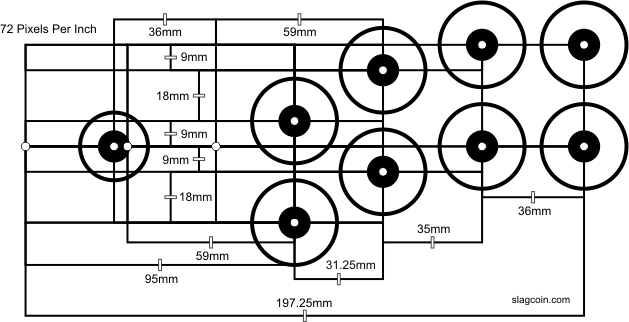
\includegraphics[width=1.0\linewidth]{hori36_s.png}
    \caption{Standard Japanese Arcade Button Layout\cite{panellayout}}
    \label{fig:buttonlayout}
\end{figure}



\section{Research Method and Computing Component}
To be able to properly assess player's inputs and the speed at which they do so, my computing component will be an input capturing program that will be written in C++ and pull in data from Microsoft's XINPUT library as that can be accessed from a C++ program with relative ease, this program will time stamp all of the inputs from both players so that I can assess how quickly they can input say, a certain combo and just in general play, so that I can access the different input methods affect player's while looking at the other factors that may impact their results, such as palm width and fore finger length, as this was covered in another paper I found\cite{omichands} and it would be good to cross compare with what they found and how it affected players. Another metric that I feel would be useful to look at would be the time it takes to beat the AI opponent, as this is how I intend on keeping my data consistent as an AI opponent is a lot more uniform than having two subjects play against each other; this data can then be used to side by side compare the different control methods and draw conclusions based on that. To maintain a standard for timing the matches, I feel that using screen capturing software would be the best option as it captures the in-game timer, this also brings the advantage of being able to study the gameplay, which allows me to make much more informed observations.

\section{Hypothesis}

Insert more sections here.
Use BibTeX~\cite{bibtex} to cite relevant literature.

\section{Conclusion}
The conclusion goes here.

% references section

\bibliographystyle{IEEEtran}
\bibliography{references}

% Appendices

\appendices
\section{First appendix}
Appendices are optional. Delete or comment out this part if you do not need them.

% that's all folks
\end{document}
